\section{Инструкции по восстановлению последовательности 1С Розница}

\subsection{Введение}

\begin{itemize}
	\item Для корректного формирования и просмотра отчетов о себестоимости необходимо учитывать следующее: ,,границу последовательности`` и ,,дату запрета редактирования документов``. Для того что бы получить правильную себестоимость товара, документы участвующие в её формировании должны быть проведены в строго хронологической последовательности.
	Любое проведение документа ,,задним`` числом нарушает границу последовательности и требуется её восстановления. ,,Дата запрета редактирования документов`` позволяет запретить проводить документы в ,,закрытом`` периоде, за который будут формироваться отчеты и препятствует нарушению границы последовательности.
\end{itemize}	
\begin{enumerate}	
	\item Обработка восстановления последовательности находится в разделе ,,Склад`` Рис.~\ref{ris:1.jpg}
	\begin{figure}[H]
		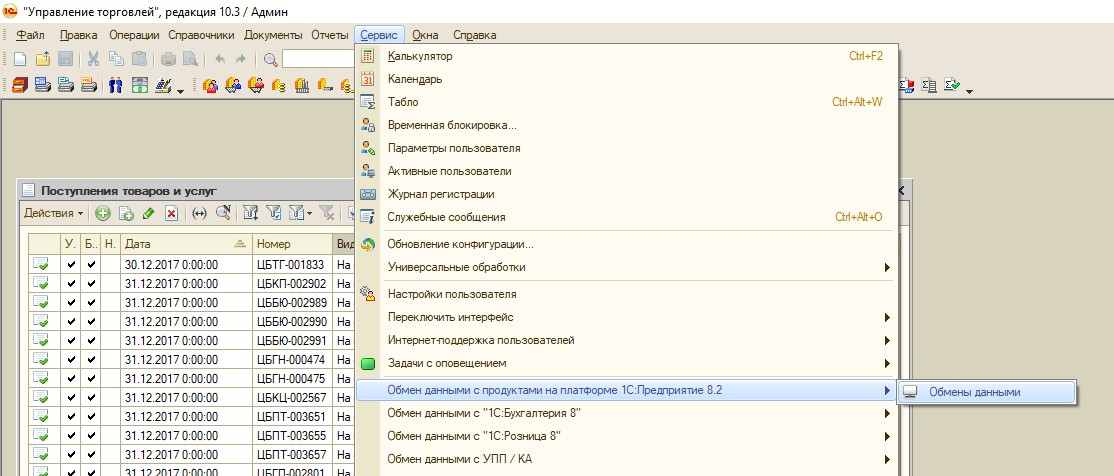
\includegraphics[width=0.7\textwidth]{1.jpg}
		\caption{Расположение в разделе ,,Склад``.}
		\label{ris:1.jpg}
	\end{figure}
	\item Для открытия обработки необходимо выбрать пункт ,,Дополнительные обработки``	
	В этой форме нас интересует пункт ,,Дополнительные обработки`` Рис.~\ref{ris:2.jpg}
	\begin{figure}[H]
		\center{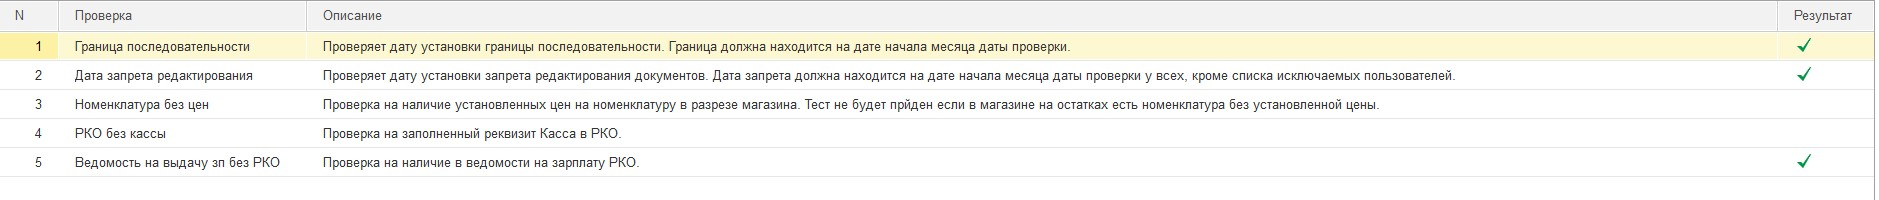
\includegraphics[width=.7\linewidth,keepaspectratio]{2.jpg}}
		\caption{Дополнительные обработки.}
		\label{ris:2.jpg}
	\end{figure}
	\item Выбрать этот пункт, откроется окно с внешними обработками Рис.~\ref{ris:3.jpg}	
	\begin{figure}[H]
		\center{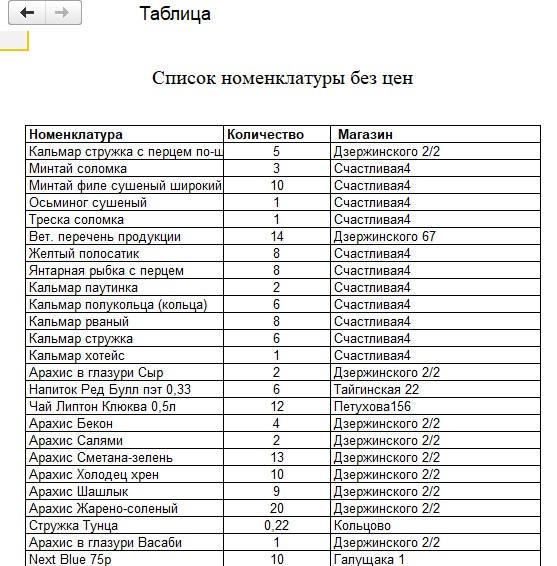
\includegraphics[width=.7\linewidth,keepaspectratio]{3.jpg}}
		\caption{,,Внешние обработки``.}
		\label{ris:3.jpg}
	\end{figure}
	\item Выбрать  обработку  ,,Проведение документов``.  И нажать ,,Выполнить`` Рис.~\ref{ris:4.jpg}	
	\begin{figure}[H]
		\center{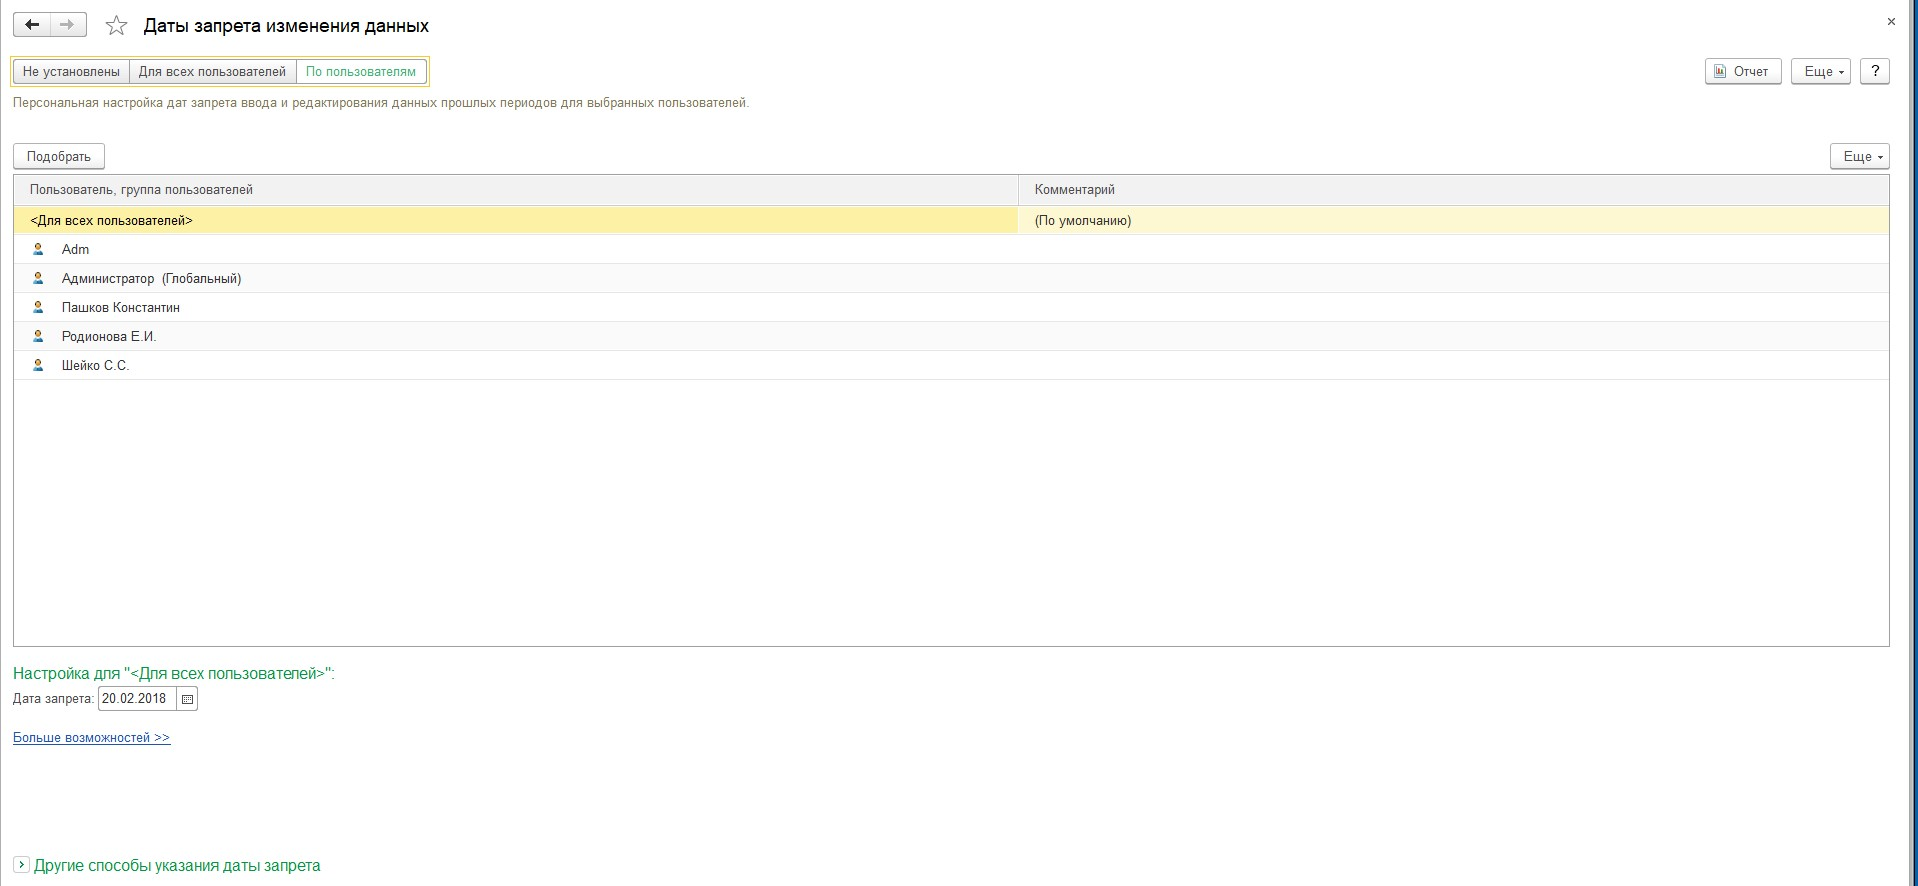
\includegraphics[width=.7\linewidth,keepaspectratio]{4.jpg}}
		\caption{Выбор проведения документов.}
		\label{ris:4.jpg}
	\end{figure}
	\item В открывшейся форме ,,Проведение документов`` выбрать вкладку ,,Восстановление последовательности`` Рис.~\ref{ris:5.jpg} 
	\begin{figure}[H]
		\center{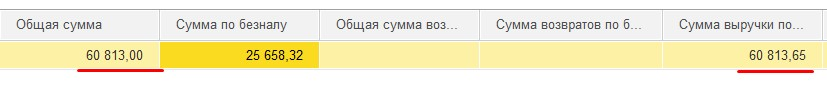
\includegraphics[width=.7\linewidth,keepaspectratio]{5.jpg}}
		\caption{Выбор вкладки.}
		\label{ris:5.jpg}
	\end{figure}
	\item Имеется возможность задать дату по до какой восстанавливать последовательность. Если дату не задавать, 
		  то последовательность будет восстановлена на дату последнего документа (в общем случае по текущую дату) Рис.~\ref{ris:5_1.jpg} 
	\begin{figure}[H]
		\center{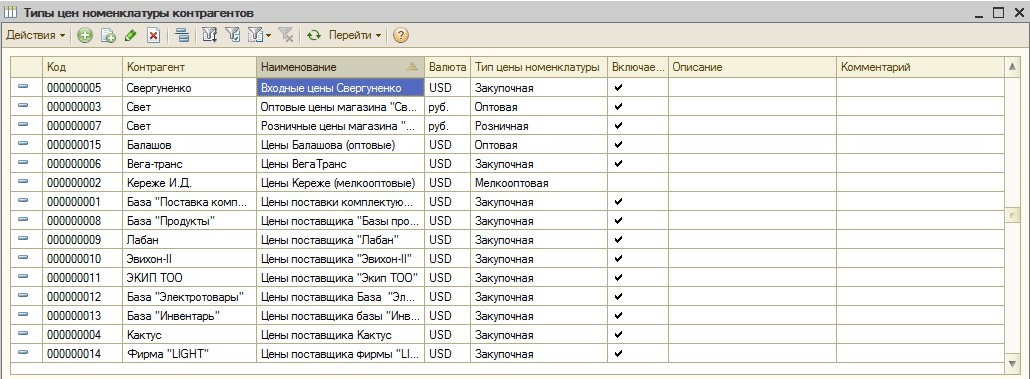
\includegraphics[width=.7\linewidth,keepaspectratio]{5_1.jpg}}
		\caption{Установка даты.}
		\label{ris:5_1.jpg}
	\end{figure}
	\item В колонке ,,Граница`` можно увидеть на какую дату установлена последовательность в текущий момент. Нажатие кнопки ,,Восстановить`` запускает процесс восстановление последовательности. Рис.~\ref{ris:6.jpg} 
	\begin{figure}[H]
		\center{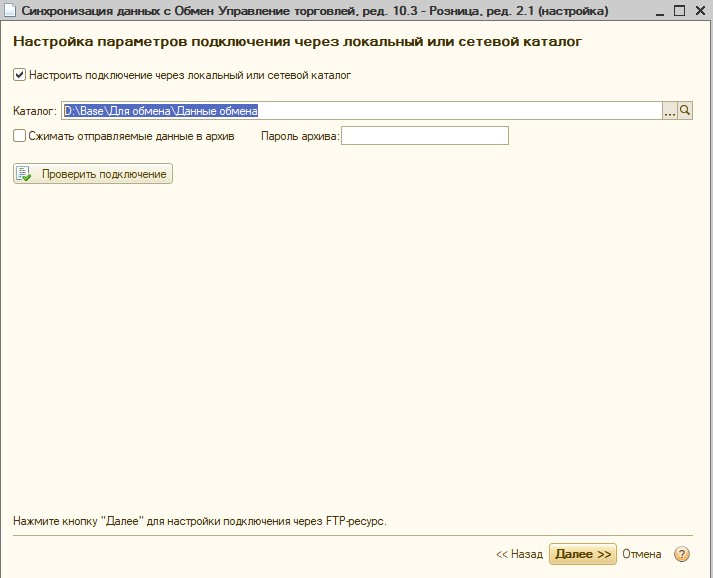
\includegraphics[width=.8\linewidth,keepaspectratio]{6.jpg}}
		\caption{Восстановление последовательности.}
		\label{ris:6.jpg}
	\end{figure}
	\item Внимание! Восстановление последовательности может занять длительное время.
	\end{enumerate}

\subsection{При возникновении ошибок}
	Есть несколько типов ошибок возникающих при восстановлении последовательности:
\begin{itemize}
\item Ошибки связанные с некорректными данными в документах. Это \underline{ошибки Проведения документа}  При ошибках подобного рода, необходимо открыть документ, выполнить проведение документа ,,руками``, посмотреть ошибки.Исправить их. Добиться того, что бы проведение документа стало успешным. Продолжить восстановление последовательности.\par При ошибках этого типа в диагностических сообщениях обычно содержится номер и тип документа в, который не удалось провести. 	
\item Ошибки связанные с  механизмом восстановления последовательности или ошибки 1С.\par Сообщения об ошибках этого типа могут не содержать понятной для пользователя информации. При их возникновении необходимо сделать ,,скриншот`` экрана и отправить его на почту тех.поддержки.   	



\end{itemize}		